\chapter{Einleitung}
\section{Motivation}
Motiviert wurde diese Arbeit durch das Paper \cite{doi:10.1021/acsnano.1c00139}.
In dem dort behandelten Experiment wird mittels ultralow-energy ion implantation Mangan (Mn) in eine einzelne Graphenstörstelle, wobei sich das Graphen auf einem Kupfersubstrat befindet, eingesetzt.
Es wurden die Positionen des Mangans im Bezug auf die Moiré Superstruktur (Abbildung \ref{fig:ascnano_structure}), die elektronischen und magnetischen Eigenschaften und die Konzentration der Mangan-Defekte
untersucht.
Die Moiré Superstruktur bildet sich aus, da die vertikale Ausrichtung zwischen dem Graphen und dem Kupfer kontinuierlich variiert.
Graphen mit Manganstörstellen eignet sich für die Untersuchung elektrischer und magnetischer Eigenschaften, da es bei einer Konzentration von ca. $\qty{0.04}{\percent}$ 
die Dirac-ähnlichen Bänder beibehält und es somit ein ideales System für das Studieren der Interaktion
zwischen lokalen magnetischen Momenten und den Diracelektronen darstellt.
Abbildung \ref{fig:ascnano_structure}(a) zeigt die Probe auf atomarer Ebene, worin auch die Moiré Superstruktur dargestellt ist.
Die Stellen mit hoher Symmetrie bezüglich des Stapelns des Graphens auf dem Substrat werden in 
Abbildung \ref{fig:ascnano_structure}(b-d) aufgezeigt.
\begin{figure}
    \centering
    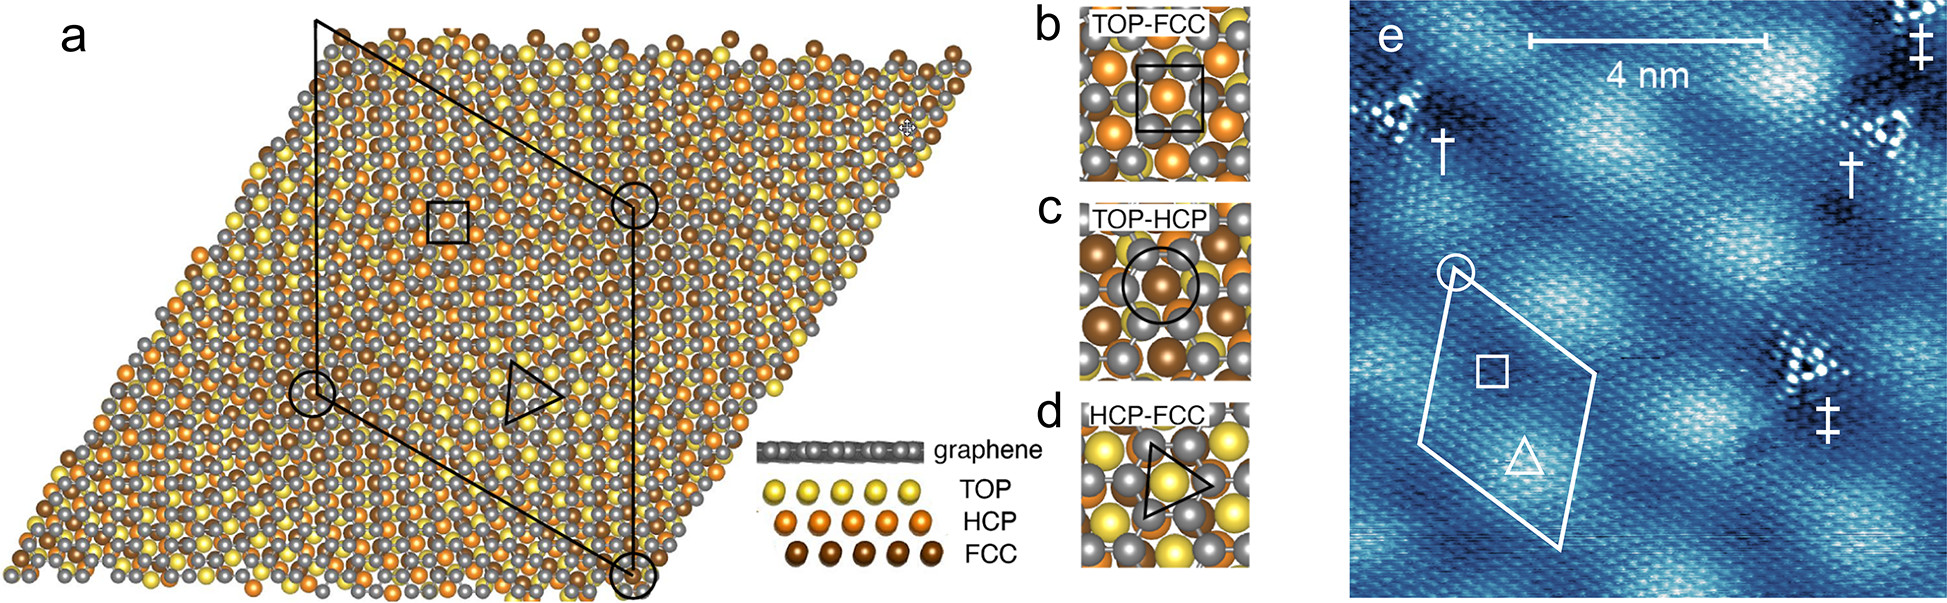
\includegraphics[width = \textwidth]{Plots/images_large_nn1c00139_0002.jpeg}
    \caption{(a) zeigt die Moiré Superstruktur. Durch kontinuierliche Variation der der Ausrichtung 
    zwischen dem Kupfer und Graphen, entstehen Hochsymmetriepunkte bezüglich des Stapelns (b-d).
    Diese Hochsymmetriepunkte und somit auch die Moiré Superstruktur können mittels RTM 
    visualisiert werden, womit eine zweidimensionale Periodizität ersichtlich wird (e).
    (Abbildung entnommen aus \cite{doi:10.1021/acsnano.1c00139})}
    \label{fig:ascnano_structure}
\end{figure}
Diese bilden wiederrum ein zweidimensionales Gitter (Abb. \ref{fig:ascnano_structure}(e)).
Ebenfalls ist die vertikale Position des Manganatoms von Relevanz, da aufgrund der kurzen Reichweite der Bindungen,
welche Graphen charakterisiert, und des großen Radius von Mangan im Vergleich zur Kohlenstofffehlstelle das Manganatom senkrecht zur Graphenebene
entweicht.
Dieses kann sich zwischen das Graphen und das Substrat oder zwischen Graphen und Vakuum (nach außen gerichtet) entweichen. 
Jedoch wurden mögliche nach außen gerichtete Anordnung nur mit einer Wahrscheinlichkeit, 
welche um zwei Größenordnungen kleiner ist, beobachtet.
Dies lässt sich mit der Tatsache erklären, dass die Konfiguration mit dem nach außen gerichteten Manganatom
eine höhere Energie aufweist und somit instabiler ist.
\begin{figure}
    \centering
    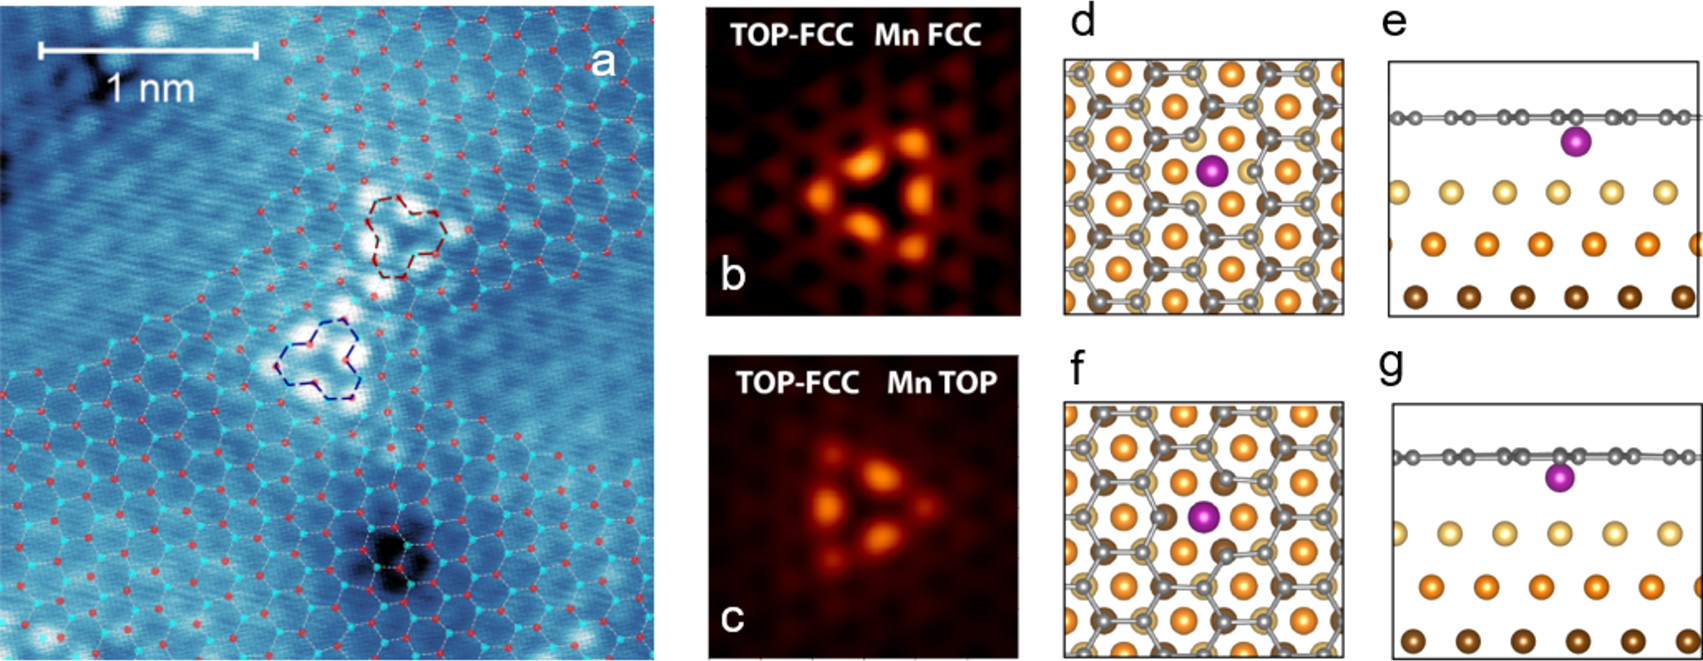
\includegraphics[width = \textwidth]{Plots/images_large_nn1c00139_0003.jpeg}
    \caption{(a) zeigt eine RTM, wo Mangan auf den beiden verschiedenen Untergittern von Graphen implantiert wurde. In der
    RTM äußern sich diese mittels dreieckigen Strukturen, welche zueinander gespiegelt liegen.
    (b-c) zeigen RTM simuliert mittels DFT um TOP-FCC Stapeln. In (b) liegt das Mn-Atom auf einem FCC
    und in (c) auf einem TOP Gitterplatz. (d-g) zeigen die Anordnung des Manganatoms respektive des Gitterplatzes
    in der Graphenebene und seitlich davon. 
    (Abbildung entnommen aus \cite{doi:10.1021/acsnano.1c00139})}
    \label{fig:ascnano_defect}
\end{figure}
\section{Eigenschaften von Graphen}
Graphen ist ein zweidimensionales, aus einer Atomschicht bestehendes Allotrop von Kohlenstoff (Cu), angeordnet in einem hexagonalen
Bravais-Gitter. 
Der größte Teil der Bindung geht von den $sp^2$-Hybridorbitalen aus, welche eine $\sigma$-Bindung eingehen, so dass 
die die Bindungspartner in einem Winkel vom $\ang{120;;}$ zueinander liegen. 
Das zu der Graphenebene senkrecht liegende p-Orbital sorgt mit dessen $\pi$-Bindung für eine gute Leitfähigkeit.\cite{graphene_properties}
Eine $\sigma$ und eine $\pi$-Bindung sorgen für eine Doppelbindung.
Graphen ist aufgrund dessen Eigenschaften von großem Interesse und ein aktuelles Forschungsthema.
Einerseits ist die  Dichte mit $\qty{0.77}{\milli\gram\per\metre\squared}$ extrem gering, obwohl 
Graphen eine hundertfache Stärke von Stahl bei der selben Dicke aufweist.\cite{graphene_properties} 
Anderseits ist Graphen das bisher bekannte am besten leitende Material bei Raumtemperetur mit einer Leitfähigkeit von 
$\qty{e6}{\siemens\per\metre}$\cite{graphene_properties}. 
Dies lässt sich mit den Elektronen aus den schwachen $\pi$-Bindungen erklären, welche sich frei bewegen können.
Außerdem sind die Bänder mit der Dispersionsrelation
\begin{equation*}
    \epsilon_{\vec{k}} \propto \pm \sqrt{3+2\cos(\sqrt{3}ak_y)+2\cos(\frac{3}{2}ak_x+\frac{\sqrt{3}}{2}ak_y) + 2\cos(\frac{3}{2}ak_x-\frac{\sqrt{3}}{2}ak_y) }
\end{equation*}
und der Form eines Kegels nennenswert.
Das negative bzw. positive Vorzeichen gehört zu dem Valenz- bzw. Leitungsband. 
Die Bänder berühren sich and den Diracpunkten\footnote{An den Diracpunkten ist die Dispersionsrelation null.}, wodurch ein Austausch von Elektronen auch bei verschwindender thermischer Anregung 
stattfinden kann.\cite{graphene_properties}
\section{Struktur von Graphen und der Störstelle}
\label{sec:structure}
Die Struktur von Graphen kann nur mit einer zweiatomigen Basis beschrieben werden, da sonst keine Translationsinvarianz vorherrschen würde.
Dazu kann das Kristallgitter in zwei Gitter (A und B) aufgeteilt werden.
Die in der Abbildung \ref{fig:graphene_lattice} eingezeichneten Nächsten-Nachbarn-Vektoren können durch einen Drehwinkel $\varphi_i$ beschrieben werden, so dass sich 
mit dem Gitterabstand a
\begin{equation*}
    \vec{\delta}_i(\varphi_i) = a\begin{pmatrix} \sin (\varphi_i) \\ \cos (\varphi_i)     \end{pmatrix}
\end{equation*}
ergibt.
Wird das Koordinatensystem so gelegt, so dass $\vec{\delta}_1$ auf der x-Achse liegt, lassen sich die Abstandsvektoren mittels 
\begin{equation*}
    \vec{\delta}_1 = a \begin{pmatrix} 1            \\[4pt] 0                   \end{pmatrix}, \quad
    \vec{\delta}_2 = a \begin{pmatrix} -\frac{1}{2} \\[4pt] \frac{\sqrt{3}}{2}  \end{pmatrix}, \quad 
    \vec{\delta}_3 = a \begin{pmatrix} -\frac{1}{2} \\[4pt] -\frac{\sqrt{3}}{2} \end{pmatrix}
\end{equation*}
darstellen. \\
\begin{figure}
    \centering
    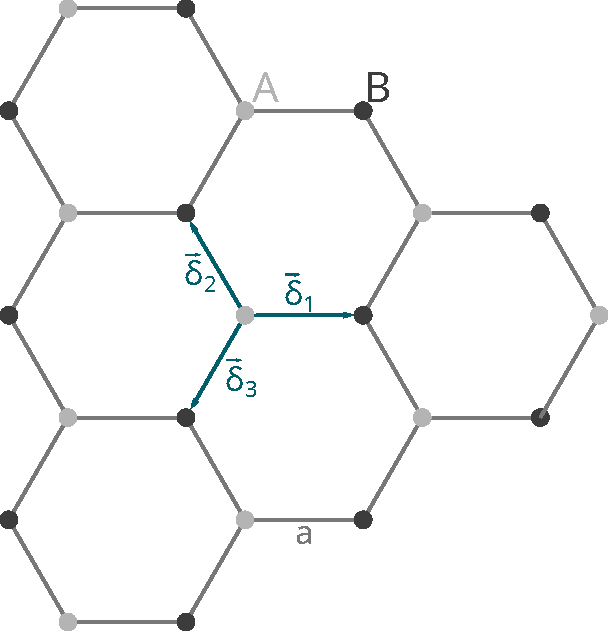
\includegraphics[width = 0.5\textwidth]{Plots/graphene_lattice.pdf}
    \caption{Honigwabengitter von ungestörtem Graphen mit eingezeichneten Nächste-Nachbar-Vektoren.}
    \label{fig:graphene_lattice}
\end{figure}
Wird nun ohne Beschränkung der Allgemeinheit ein Kohlenstoffatom aus dem Untergitter A entfernt und dort ein Manganatom eingesetzt, ändern sich die
Abstandsvektoren. 
Dies liegt daran, dass das Manganatom zu groß ist und nicht in diese Stelle passt, so dass es aus der Ebene entweicht und eine $z$-Komponente besitzt.
Diese Situation ist in Abbildung \ref{fig:mangan_impurity} dargestellt.
\begin{figure}
    \begin{subfigure}{0.48\textwidth}%
    \centering%
    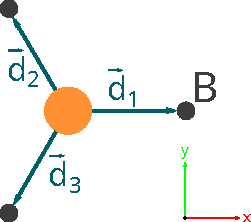
\includegraphics[height=3cm]{Plots/mangan_impurity_inplane.pdf}%
    \caption{Mangandefekt in Graphen betrachtet in Graphenebene.}%
    \label{fig:mangan_impurity_inplane}%
    \end{subfigure}%
    \hfill% Fills available space in the center -> space between figures
    \begin{subfigure}{0.48\textwidth}%
    \centering%
    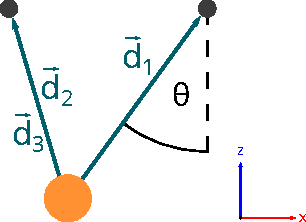
\includegraphics[height=3cm]{Plots/mangan_impurity_z_component.pdf}%
    \caption{Manganstörstelle dargestellt in einer seitlichen Ansicht.}%
    \label{fig:mangan_impurity_z_component}%
    \end{subfigure}%
    \caption{Darstellung des räumlichen Anordnung des Mangandefekts aus veschiedenen Ansichten.}%
    \label{fig:mangan_impurity}%
\end{figure}%
Wie bereits in Abbildung \ref{fig:mangan_impurity} angedeutet, wird im folgenden angenommen, dass das Mangan mittig von den nächsten Nachbarn liegt, so dass 
sich die $x$- und $y$-Komponente der Abstandsvektoren nicht ändert.
Lediglich haben die Abstandsvektoren bei Betrachtung des Mangandefekts eine zustäzliche z-Komponente.
Diese $z$-Komponente lässt sich mittels trigonometrischen Beziehungen zu $z = -\cot (\theta)$ bestimmen, womit die 
Abstandsvektoren durch 
\begin{equation*}
    \vec{\delta}_1 = a \begin{pmatrix} 1            \\[4pt] 0                   \\[4pt] \cot (\theta)\end{pmatrix}, \quad
    \vec{\delta}_2 = a \begin{pmatrix} -\frac{1}{2} \\[4pt] \frac{\sqrt{3}}{2}  \\[4pt] \cot (\theta)\end{pmatrix}, \quad 
    \vec{\delta}_3 = a \begin{pmatrix} -\frac{1}{2} \\[4pt] -\frac{\sqrt{3}}{2} \\[4pt] \cot (\theta)\end{pmatrix}
\end{equation*}
angegeben werden können. 
In dieser Arbeit wird nur der Überlapp zwischen den 5 $3d$-Orbitalen des Manganatoms und den $p_z$-Orbitalen der umliegenden Kohlenstoffatome betrachtet.